\section{Kompressionsverfahren der Feldlinien} \label{konzept}
konzept der unterschiedlichen kompressionsverfahren. zwei lösungsansätze. 
bereits eine simple Kompression implementiert.

\subsection{Ist-Komprimierung} \label{konzept:ist-komprimierung}
\begin{figure}[!htbp]
	\center
	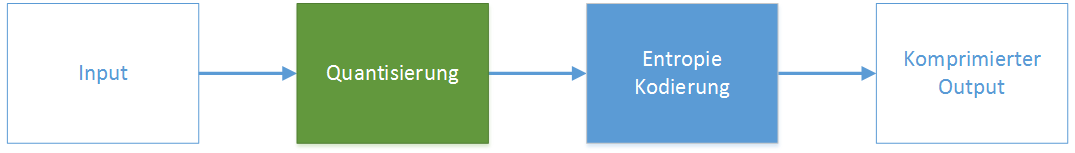
\includegraphics[width=0.8\textwidth,height=6cm,keepaspectratio]{./pictures/konzept/ist/aufbau.png}
	\caption{Aufbau der Ist-Kompression.}
	\label{konzept:ist:aufbau:diagramm}
\end{figure}
Das Ziel der Ist-Kompression ist es, die Datenmenge mit einfachen Mitteln drastisch zu reduzieren. Der Aufbau ist im Diagramm der Abbildung \ref{konzept:ist:aufbau:diagramm} dargestellt. Die Ist-Kompression führt zuerst ein Subsampling durch. Drei Viertel aller Punkte werden in diesem Schritt verworfen. Im nächsten Schritt werden die übrigen Punkte  auf 16-Bit Integer diskretisiert. Das reduziert die Anzahl Bytes und verbessert die Kompression im Schritt Entropie Kodierung. Die Implementationen der Entropie Kodierer scheinen Integer-Werte einfacher komprimieren zu können. In der Entropie Kodierung werden die Daten geordnet wie in Tabelle \ref{konzept:ist:entropie} dargestellt.
\begin{table}[!htbp]
	\center
	\begin{tabular}{|c|c|c|c|}
	\hline
	Anzahl Punkte der Feldlinien & X Kanal aller Punkte & Y Kanal aller Punkte & Z Kanal aller Punkte \\\hline
	\end{tabular}
	\caption{Anordnung der Simulationsdaten der Ist-Kompression}
	\label{konzept:ist:entropie}
\end{table}
Als erstes werden die Längen aller Feldlinien abgelegt. Danach folgt der X, Y und der Z Kanal aller Punkte der Feldlinien. Diese Anordnung verbessert die Kompressionsrate der Entropie Kodierung. Je näher ähnliche Muster beieinander liegen, desto besser können sie Komprimiert werden. Für die eigentliche Entropie-Kodierung wird Gzip verwendet. Gzip basiert auf dem Deflate Algorithmus, welcher aus einer Kombination von LZ77 und Huffman Kodierung besteht \cite{wiki:gzip}.\\
Die Punktmenge ist für Low-End Grafikkarten zu gross. Um die Punktmenge für die Visualisierung zu verkleinern, führt der JHelioviewer ein weiteres Subsampling durch, welches im Abschnitt \ref{konzept:loesung0:subsampling} beschrieben ist.

\subsection{Lösungsansatz: Adaptives Subsampling} \label{konzept:loesung0}
\begin{figure}[!htbp]
	\center
	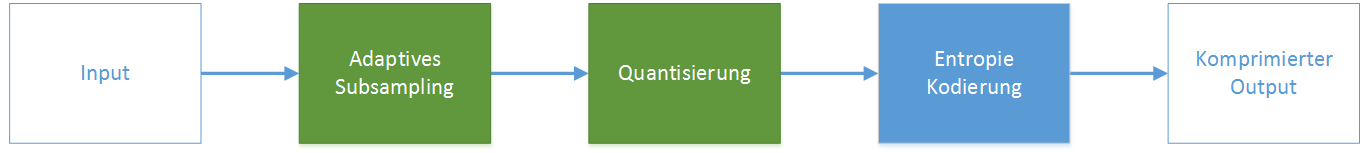
\includegraphics[width=0.8\textwidth,height=6cm,keepaspectratio]{./pictures/konzept/solution0/aufbau.png}
	\caption{Aufbau des Lösungsansatzes: Adaptives Subsampling.}
	\label{konzept:loesung0:aufbau:diagramm}
\end{figure} 
Dieser Lösungsansatz verwendet einen ähnlichen Aufbau wie die Ist-Kompression \ref{konzept:ist-komprimierung}. Der Unterschied ist, dass das Subsampling Verfahren gewählt wurde, welches der JHelioviewer auf dem Client durchführt. Die Abbildung \ref{konzept:loesung0:aufbau:diagramm} zeigt den neuen Ablauf.\\
Dieser Ansatz überträgt nur die Information, die der JHelioviewer zur Visualisierung benötigt. Der Vorteil ist dass die Information, die der JHelioviewer visualisiert ein Bruchteil darstellt und somit eine hohe Kompressionsrate ereicht werden kann. Es ist möglich dass die Visualisierung zu einem späteren Zeitpunkt mehr Punkte darstellen soll. In diesem Fall müssten entweder mehr Punkte übertragen werden, was eine schlechtere Kompressionsrate zur Folge hat, oder der JHelioviewer muss eine Interpolation durchführen. 

\subsubsection{Adaptives Subsampling}\label{konzept:loesung0:subsampling}
Konzeptionell approximiert das adaptive Subsambling eine Kurve diruch eine Folge von Strecken. Je stärker die Krümmung der Kurve, desto mehr Strecken werden für die Approximation benötigt.
\begin{figure}[!htbp]
	\center
	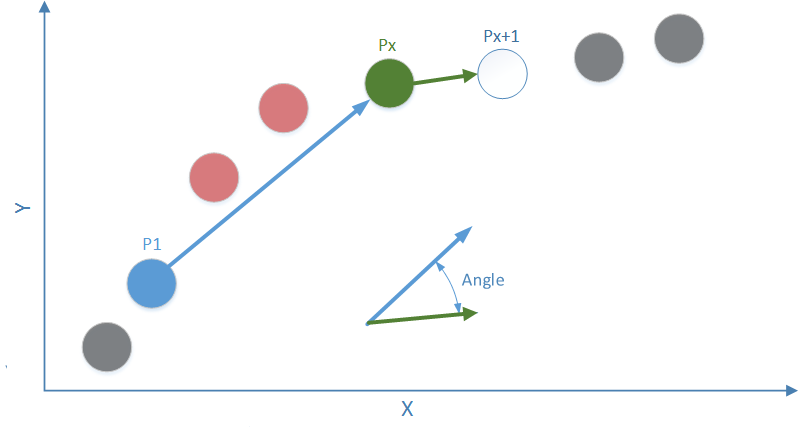
\includegraphics[width=0.8\textwidth,height=6cm,keepaspectratio]{./pictures/konzept/solution0/anglesubsampling.png}
	\caption{Darstellung des Adaptiven Subsapmlings im 2D Raum. Rot sind die Punkte, welche geprüft und gelöscht wurden. Grün ist der Punkt dargestellt, welcher geprüft wird.}
	\label{konzept:loesung0:angle}
\end{figure}
Das Diagramm der Abbildung \ref{konzept:loesung0:angle} stellt das Subsampling im zweidimensionalen Raum dar. Das Adaptive Subsampling wählt nun Punkte $P$ aus der Feldlinie aus, welche Start- und Endpunkte der Strecken darstellen.\\
$P_1$ wurde bereits ausgewählt. Es wird nun ein Punkt $P_x$ gesucht, der als Endpunkt einer Strecke von $P_1$ zu $P_x$ die Feldlinie approximiert. Dazu wird der Winkel der Strecke $P_1$ zu $P_x$ mit der Strecke $P_x$ zu $P_x+1$ verglichen. Wenn der Winkel kleiner ist, als ein Winkel $\alpha$, wird der nächste Punkt $P_x+1$ überprüft. Wenn der Winkel grösser ist, wird $P_x$ ausgewählt. Danach wird der wird eine nächste Strecke startend von $P_x$ gesucht.

\subsubsection{Entropie Kodierung mittels RAR} \label{konzept:loesung0:kodierung}
Die Anordnung der Daten wurde aus der Ist-Kompression übernommen, jedoch wird Rar anstatt GZip verwendet. GZip konnte bei den Ist-Komprimierten Daten eine Kompressionsrate von $1.2$ erreichen, während Rar bei selben Daten eine Rate von $3.7$ erreicht.
\pagebreak

\subsection{Lösungsantz: Diskrete Kosinus Transformation}\label{konzept:loesung1}
\begin{figure}[!htbp]
	\center
	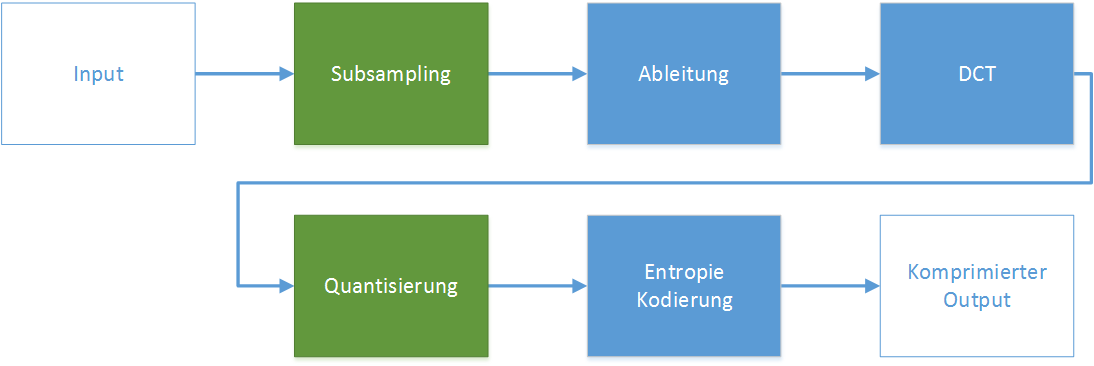
\includegraphics[width=0.8\textwidth,height=6cm,keepaspectratio]{./pictures/konzept/solution1/aufbau.png}
	\caption{Aufbau des Lösungsansatzes: Adaptives Subsampling.}
	\label{konzept:loesung1:aufbau}
\end{figure} 
Die Kompression dieses Lösungsansatzes ist Dargestellt im Diagramm der Abbildung \ref{konzept:loesung1:aufbau}. Konzeptionell ähnelt dieser Ansatz der JPEG/JFIF Kompression (dargestellt in der Abbildung \ref{state:jpeg:abb}), die einzelnen Teilschritte können aber andere Algorithmen verwenden. Im Vergleich zum JPEG/JFIF Standard ist der grösste Unterschied, dass das Eingangssignal vor der Kosinus Transformation abgeleitet wird.

Die Feldlinien ähneln oft harmonischen Halbwellen, welche sich durch wenige Kosinusfunktionen approximieren lassen können. Um eine optimale Kompression mit dieser Variante zu erreichen, müssen Ringing Artefakte \cite{wiki:ringing:artefacts} behandelt werden. Sie äussern sich als Oszillieren im dekomprimierten Signal, was das menschliche Auge als störend empfindet. Beispiele für die Ringing Artefakten von Feldlinien sind im Abschnitt \ref{resultate:loesung1:ringing} zu finden.\\
Es gibt Möglichkeiten, die Ringing Artefakte zu Dämpfen oder gar zu beheben: Die simpelste Variante ist es, das dekomprimierte Signal zu glätten. Die Glättung kann das Signal verfälschen und ist deshalb nicht die optimale Lösung. In der Bild- und Audioverarbeitung wird aktiv nach Filter geforscht, welche die Ringing Artefakte in der Dekompression vermindern \cite{kaup1998reduction} \cite{park1999postprocessing}.

\subsubsection{Subsampling} \label{konzept:loesung1:subsampling}
Das Subsampling wurde aus der Ist-Kompression \ref{konzept:ist-komprimierung} übernommen und dient, die DCT zu beschleunigen. Da die DCT eine Komplexität von $O(n^2)$ aufweist, wird durch das Subsampling die Transformation wesentlich beschlenuitgt.\\
Falls die Laufzeit der Dekompression weiter verbessert werden soll, kann die Fast-Cosine-Transformation umgesetzt werden. Diese hat eine Komplexität von $O(n log(n))$. Falls das nicht ausreicht, können die Linien in Blöcke unterteilt werden und die DCT pro Block ausführen. Dadurch wird die Komplexität auf $O(n)$ gesenkt. Jedoch ist es wahrscheinlich, dass durch die Unterteilung die Kompressionsrate leidet. Die Approximation mehrer Blöcke des Eingabesignals benötigt schlussendlich mehr Kosinusfunktionen, als die Approximation des gesamten Signals.

\subsubsection{Ableitung}
Das Eingabesignal wird abgeleitet und alle folgenden Transformationen werden auf den Steigungen des Signals ausgeführt. Damit die Transformation umkehrbar ist, muss der Startpunkt zusätzlich abgespeichert werden.\\
Die Artefakte, welche das abgeleitete dekomprimierte Signal beinhaltet, sind bei der Feldliniensimulation weniger störend für das menschliche Auge. Die Feldlinie bleibt tendenziell glatt und Artefakte äussern sich meist in veränderten Amplituden, welche erst erkennbar sind, wenn die Originalfeldlinie zum Vergleich bereit steht. Diese Eigenschaft wirkt sich ebenfalls auf die Ringing-Artefakte aus. Die Ableitung hat einen dämpfenden Effekt auf die Ringing Artefakte.

\subsubsection{Cosinus-Transformation} \label{konzept:loesung1:kosinus}
Die Diskrete Kosinus Transformation stellt eine endliche Menge von $N$ Datenpunkten als $N$ Kosinusfunktionen zu verschiedenen Frequenzen dar. Die Werte DCT-Koeffizienten stellt dar, wie hoch der Anteil einer bestimmten Frequenz ist im Originalsignal. Im optimalen Fall kann ein Signal durch niederfrequente Funktionen approximiert werden. Die hochfrequenten Anteile stellen Details dar, welche meist nicht relevant sind.\\
Es gibt verschiedene Möglichkeiten die Punkte zu transformieren. Hier wurde sich am JPEG/JFIF Standard orientiert, welche die DCT-II \eqref{konzept:loesung1:kosinus:formula:fdct} als Forwärts und die DCT-III \eqref{konzept:loesung1:kosinus:formula:idct} als Rückwärtstransformation verwendet \cite{wallace1992jpeg}. 
\begin{equation} \label{konzept:loesung1:kosinus:formula:fdct}
	X_k = \sum_{n=0}^{N-1}x_n*cos[\frac{\pi}{N}k(n+\frac{1}{2})] \quad k = 0, 1, \ldots, N-1
\end{equation}
\begin{equation} \label{konzept:loesung1:kosinus:formula:idct}
x_n  = \frac{1}{2}X_0 + \sum_{k=1}^{N-1}X_k*cos[\frac{\pi}{N}k(n+\frac{1}{2})] \quad n = 0,1,\ldots,N-1
\end{equation}
$N$ bezeichnet die Länge des Eingabesisignals, $x_n$ bezeichnet einen Wert im diskreten Signal und $X_k$ ist der Anteil der Frequens $k$. Ein Eingabesignal der Länge $N$ resultiert in $N$ Kosinus-Funktionen.

Die DCT transformiert ein periodisches, unendliches Signal. Um ein endliches Signal zu transformieren, wird es konzeptionell wiederholt. Die gewählten Verfahren wiederholen das Signal jeweils in umgekehrter Reihenfolge.\\
Die Wiederholung beeinflusst die Transformation nicht, wenn das Signal an den Rändern abflacht. Falls das Signal nicht abflacht, können nach der Quantisierung an den Rändern markante Artefakte auftreten. Ein Beispiel für solche Artefakte ist im Diagramm der Abbildung \ref{resultate:loesung1:dct:artefakte} im Abschnitt \ref{resultate:dct} zu sehen.

\subsubsection{Quantisierung}
In der Visualisierung werden die Feldlinien in drei Typen unterschieden: ''Sonne zu Sonne'', ''Sonne ins Weltall'' und ''Weltall zur Sonne''.  Die ''Sonne zu Sonne'' Feldlinien können besser durch Kosinusfunktionen approximiert werden und sind weniger Anfällig auf die Ringing Artefakte. Dieser Typ von Feldlinien wird deshalb stärker Quantisiert. Für die ''Sonne zu Sonne'' Feldlinien werden maximal $35$ DCT Koeffizienten abgelegt, wobei die letzten zehn Koeffizienten kaum noch Einfluss besitzen. Sie werden mit einem hohen Faktor quantisiert, sodass sie im Normalfall ebenfalls Null sind.\\
Die anderen Feldlinien benötigen mehr Koeffizienten für die Dämpfung der Ringing Artefakte. Bei ihnen liegt das Maximum bei $50$ Koeffizienten. Die Quantisierung 

\subsubsection{Entropie Kodierung}\label{konzept:loesung1:kodierung}
Um die Entropie Kodierung zu verbessern wurden zwei Byte-Kodierungen hinzugefügt. Die Kanäle werden zuerst mit der Längenkodierung und darauf folgend mit der adaptive Genauigkeit kodiert.

\textbf{Längenkodierung}\\
Die Quantisierung erlaubt nur eine maximale Anzahl an Koeffizienten. Ab dem $50$ Koeffizient, sind die Werte Null. Die Längenkodierung schneidet den Block von Null-Koeffizienten ab und fügt die Länge des Nicht-Null Blockes hinzu. Alle Längen und alle Blöcke werden zusammen abgespeichert, die Tabelle \ref{konzept:loesung1:entropie:laengenkodierung} verdeutlicht das Konzept. $n_i$ ist die Länge der Feldlinie $i$ und $x_{i,j}$ ist der $j$ DCT-Koeffizient der Feldlinie $i$.\\
\begin{table}[!htbp]
	\center
	\begin{tabular}{||c|c|c|c|c||c|c|c}
		\hline
		\multicolumn{8}{|c|}{X Kanäle}\\\hline\hline
		 \multicolumn{5}{||c||}{Block Feldlinie 0} & \multicolumn{3}{c}{\ldots} \\\hline
		$n_0$ &$x_{0,0}$ &$x_{0,1}$ & \ldots & $x_{0,n-1}$ & $n_1$ & $x_{1,0}$ & \ldots\\\hline
	\end{tabular}
	\caption{Beispiel eines abgespeicherten Kanals mit der Längenkodierung.}
	\label{konzept:loesung1:entropie:laengenkodierung}
\end{table}
Um einen Kanal zu Dekodieren, muss die Anzahl an DCT-Koeffizienten $n_i$ gelesen werden und danach Nullen Anfügen, bis die ursprüngliche Länge des Kanals erreicht wurde. Die Anzahl Punkte jeder Feldlinie ist ebenfalls gespeichert.

Die Längenkodierung ist effizient, wenn die hochfrequenten DCT-Koeffizienten einen grossen, zusammenhängenden Null-Block bilden. Im schlechtesten Fall währe der letzte DCT-Koeffizient nicht Null. In diesem Fall würde die Längenkodierung nichts abschneiden.\\

\textbf{Adaptive Genauigkeits-Kodierung}\\
Die quantisierten Koeffizienten liegen meistens zwischen $-50$ und $+50$. Acht Bit Genauigkeit reichen im Allgemeinen aus um einen Koeffizienten abzuspeichern, nur wenige Koeffizienten benötigen mehr Genauigkeit. Mit der adaptiven Genauigkeits-Kodierung sollen so wenige Bytes pro Koeffizient abgespeichert werden, wie benötigt werden. Dazu wird wie in Tabelle \ref{konzept:loesung1:entropie:adaptive} eine neue Byte-Kodierung eingeführt. Das MSB wird als ''Continue Flag'' verwendet. Wenn es gesetzt ist, gehört das folgende Byte ebenfalls zur Zahl.\\
\begin{table}[!htbp]
	\center
	\begin{tabular}{|c|c|c|c||c|c|c|c|}
	\hline
	\multicolumn{8}{|c|}{Byte}\\\hline
	Continue Flag & X & X & X & X & X & X & X \\\hline
	\end{tabular}
	\caption{Aufteilung eines Bytes der adaptiven Genauigkeitskodierung. X sind Nutz-Bits.}
	\label{konzept:loesung1:entropie:adaptive}
\end{table}
Wenn ein Kanal hauptsächlich aus tiefen Zahlen besteht, können so Bytes gespart werden, ohne Genauigkeit zu verlieren. Wenn aber der Kanal aus hauptsächlich grossen Zahlen besteht, welche zwei oder mehr Bytes an Genauigkeit brauchen, wird weniger Speicherplatz gespart.